\documentclass[border=5mm, tikz]{standalone}

\usepackage{tikz}

\begin{document}

    % Define style for nodes
    \tikzstyle{every node}=[circle, draw, fill=black!50,
    inner sep=0pt, minimum width=4pt]

    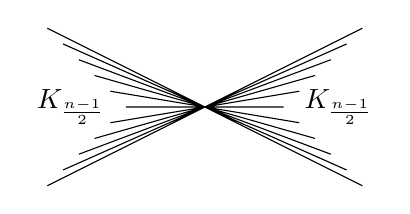
\begin{tikzpicture}[x=0.1cm,y=0.1cm]
        \draw \foreach \x in {0,2,...,10} {
        (10,0) node {} -- (-\x,\x)
        (10,0) -- (-\x,-\x)
        (10,0) -- (20+\x,\x)
        (10,0) -- (20+\x,-\x)
        };
        \node[draw=none, fill=none] at (-7,0) {$K_{\frac{n-1}{2}}$};
        \node[draw=none, fill=none] at (27,0) {$K_{\frac{n-1}{2}}$};
    \end{tikzpicture}

\end{document}